%!TEX TS-program = Arara
% arara: pdflatex: {shell: yes}
% arara: pdflatex: {shell: yes}
\documentclass[12pt,ngerman,parskip=half]{scrreprt}

% Siehe https://www.uweziegenhagen.de/?p=2928 
% für Hinweise zur Installation
% erfordert Java Runtime

\usepackage{babel}
\usepackage{blindtext}
\usepackage{graphicx}

\author{Uwe Ziegenhagen}
\title{Mein Basisdokument}

\begin{document}
\maketitle

\tableofcontents

\listoffigures

\chapter{Einleitung}

\section{Literatur}

\blindtext[2]

\blindtext[2]

\chapter{Fazit}

\begin{figure}[h]
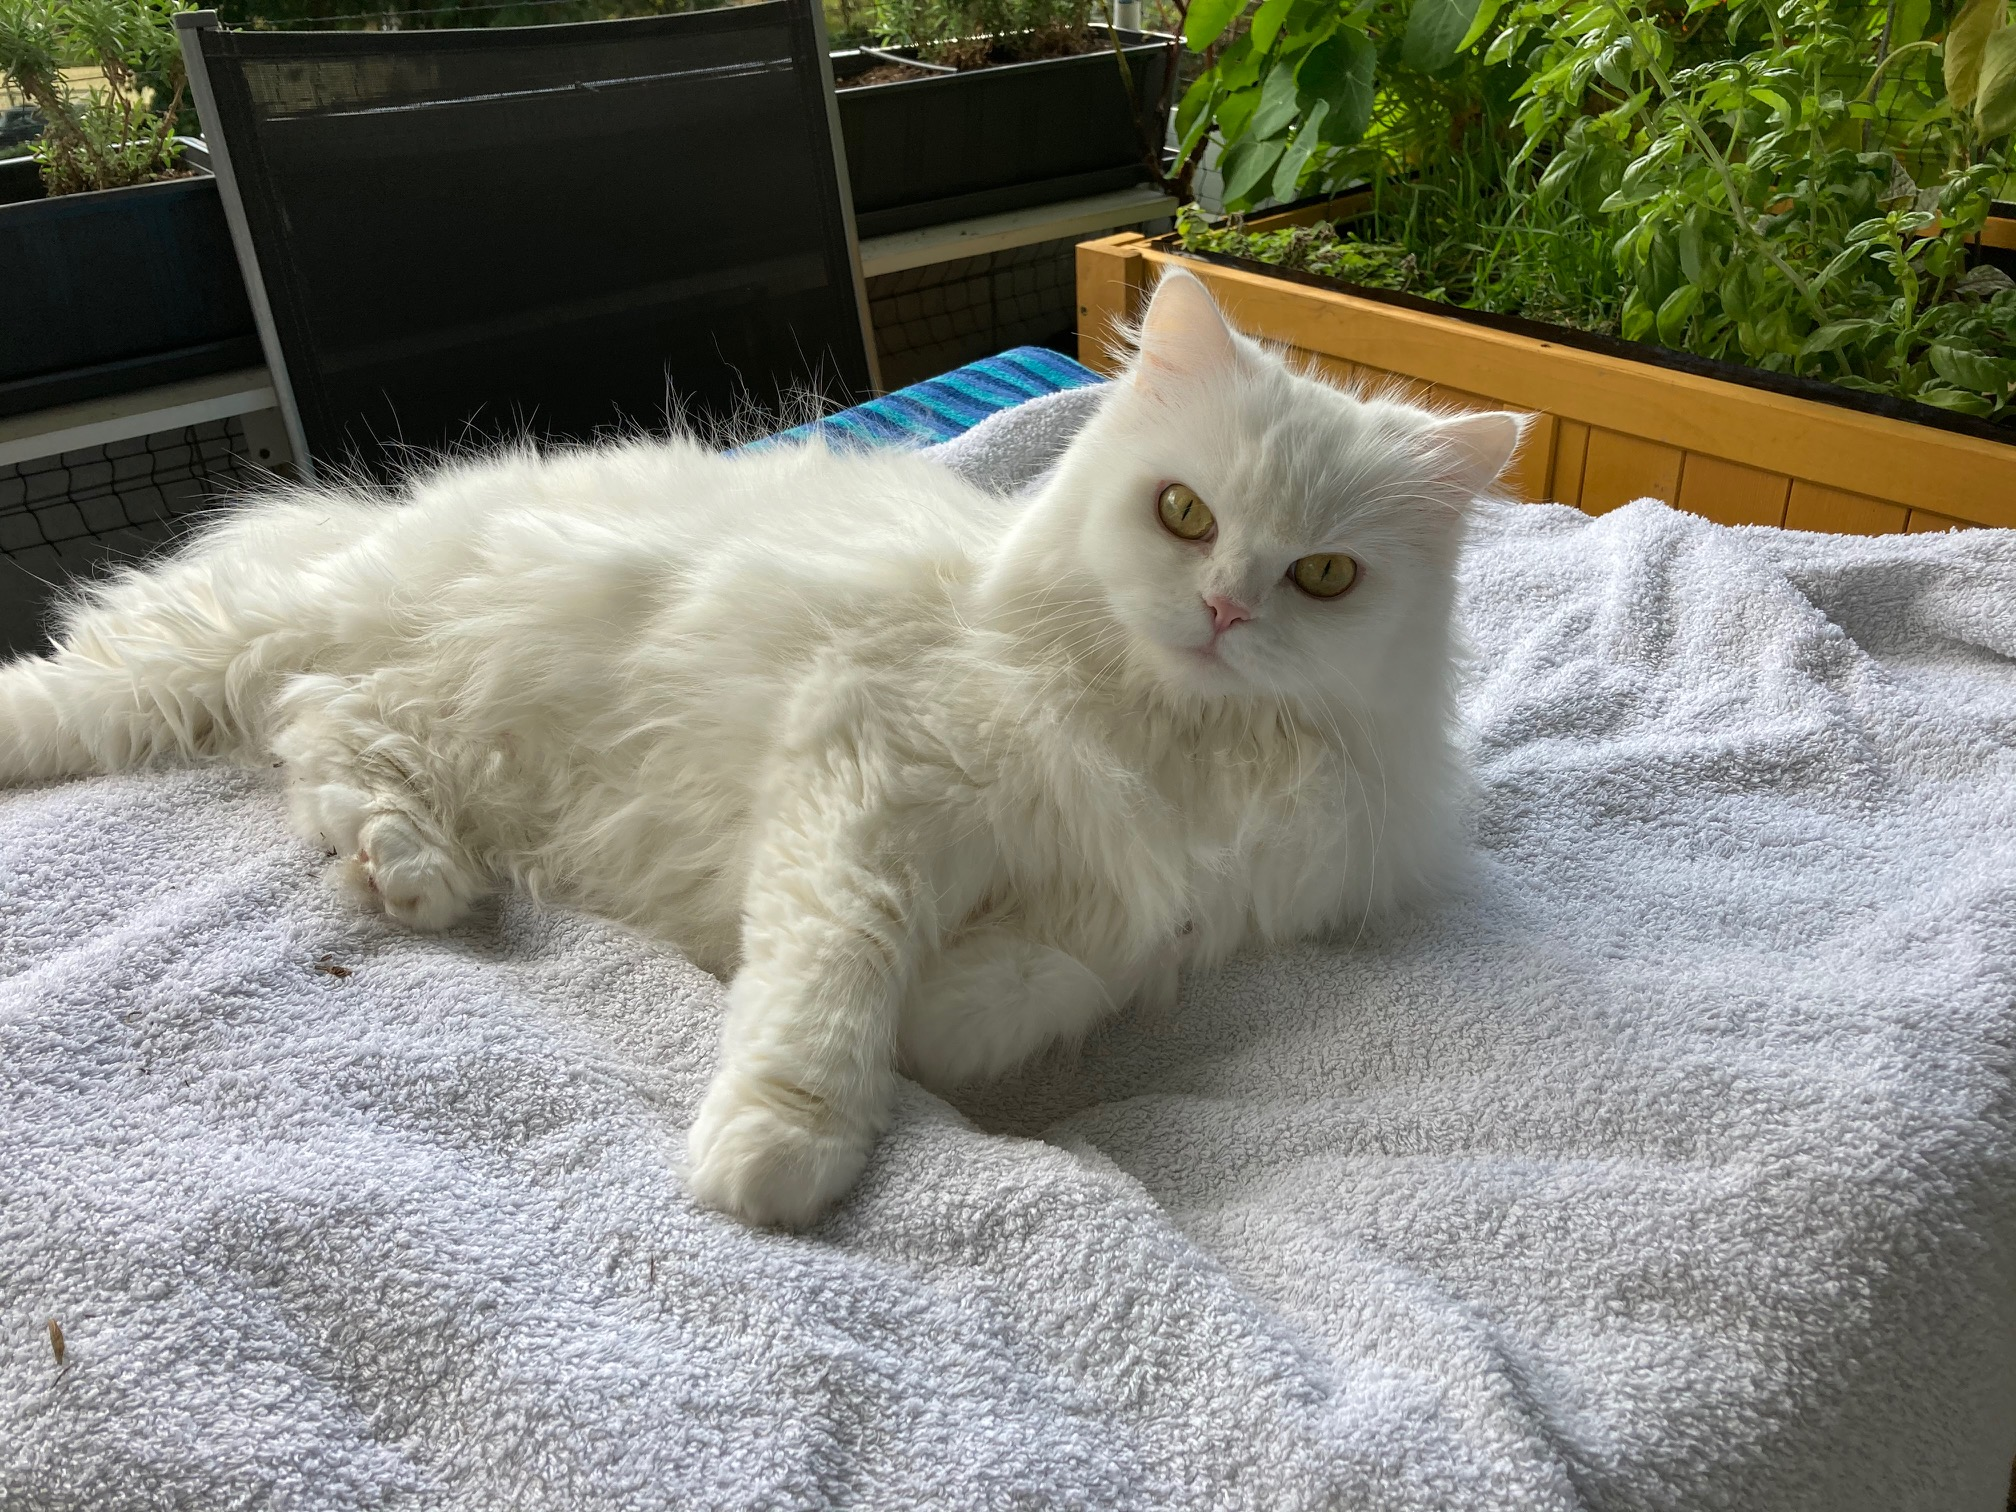
\includegraphics[width=\textwidth]{./Bilder/Katze1.jpg}
\caption{Meine Katze}
\end{figure}


\end{document}